\documentclass[dissertation.tex]{subfiles}
\begin{document}

\chapter[Identifying Optimal Biomarkers for Clinical Tests][Finding Optimal Biomarkers]{Identifying Optimal Biomarkers for Clinical Tests}
\label{chap:messina}


\emph{Thesis: Large margin binary decision stump classifiers can provide a principled way to translate research biomarker measurement data into simple but high-performance clinical tests.}


%\paragraph{Summary}
%The barrier between the research and clinical laboratory is often a major hurdle when translating research findings into clinical application.  Molecular pathology uses different measurement techniques to research, and clinical specimens are seldom as well-controlled as research ones, resulting in 
%
%A significant challenge in the translation of research findings into clinical use is the different


\section{Introduction}

Research and molecular pathology laboratories take strikingly different approaches to the measurement of biomarkers in patient samples.  Research work favours costly manual techniques, which quantify a large number of biomarkers in a relatively small number of samples.  Conversely, pathology laboratories make extensive use of highly automated turnkey systems, to robustly measure a relatively small number of biomarkers in a large number of samples.  In keeping with this divide, research and pathology laboratories often use very different technologies for the measurement of the same type of biomarker, such as RNA sequencing in research, and quantitative PCR in the clinical realm.  This difference in base technology, and the generally increased variability of clinical samples over research ones~\cite{Hewitt2008}, complicates the translation of discoveries in research into application in the clinic.

Although difficult, this translation of research discoveries into clinical practice is absolutely necessary.  Research and pathology techniques are complementary: biomarker discovery requires research techniques capable of interrogating a huge number of potential biomarkers, but the \emph{application} of any discoveries must use pathology techniques that can reliably and economically handle a potentially huge number of patient samples.  Finding effective ways to translate research findings into clinical application is critically important.  This problem can be approached from two angles: by harmonising measurement technology between research and diagnostic laboratories, or by identifying lead biomarkers in the research laboratory that have a high likelihood of effectively translating to diagnostic measurement methods.  The former approach may represent a long-term solution, but does not reflect the current state of technology.  To implement the latter approach requires bioinformatic techniques that can search large bodies of research measurement data, to identify a small number of biomarkers that are most likely to make good diagnostic tests.

Effective clinical tests must satisfy a number of requirements, which can be used to guide the translation of a research finding into a clinical tool.  Ideally, a clinical diagnostic or prognostic test should be based on the measurement of only a small number of biomarkers~\cite{Lesko2001, Pepe2001}.  Additionally, it should be highly robust to technical effects, and the inevitable variation in sample quality and handling that comes with clinical specimens~\cite{Hewitt2008}.  The results of most tests will be interpreted as a simple binary variable\footnote{For example, disease versus not diseased, responder versus non-responder, or poor prognosis versus good prognosis.}, and the detection performance of this binary variable should match the particular clinical application~\cite{Pepe2001}.  Taking all these requirements into account, a technique to translate discovery biomarker measurements into a clinical test should be able to process measurements of thousands of biomarkers, to identify those single biomarkers that, when their level is thresholded, yield a particular class separation performance, with maximal robustness to technical effects.

Existing methods for the mining of research data for potential biomarkers do not meet these requirements.  For both diagnostic and prognostic endpoints, common biomarker prioritization techniques either do not provide fine control of classification accuracy and robustness, or yield sets of biomarkers that are far too large to practically deploy.  Two broad strategies are generally employed to identify biomarkers in large research data sets: univariate statistics, and machine learning.  The first strategy encompasses approaches such as per-biomarker regression tests for association between the biomarker and a sample group or outcome, and the second covers the use of algorithms such as \glspl{SVM} to construct high-performance predictors of group or prognosis from the measurements of many biomarkers.

Univariate statistic approaches identify single biomarkers of interest, but supply no guarantee as to the suitability of these biomarkers for translation into clinical tests.  These statistics are designed to identify differences in average value between two groups, not to construct classifiers.  Significance testing and classifier learning are distinct problems, and usually have different solutions: a biomarker that shows a statistically significant difference in signal between two groups may still be a poor classifier; and vice versa (\fref{fig:messina-example-stats-class}).  Univariate tests also do not take the particular requirements of a clinical problem into account.  For example, consider two tests for the same disease -- one test is intended to be used as a population screen, and the other to rule out a suspected diagnosis.  These two tests would have very different performance requirements, and quite possibly would be best served by two different biomarkers.  Univariate test approaches to candidate biomarker selection cannot take this nuance into account, which further limits their usefulness for biomarker selection.

\begin{figure}[!htbp]
  \centering
  \vspace{1cm}
  \subbottom[Poor classification]{
    \def\svgwidth{.4\linewidth}
	\input{messina_class_test_comparison_a.pdf_tex}
    \label{fig:messina-example-stats-class-stat}}
  \hspace{1cm}
  \subbottom[Good classification]{
    \def\svgwidth{.4\linewidth}
	\input{messina_class_test_comparison_b.pdf_tex}
    \label{fig:messina-example-stats-class-class}}
  \caption[Statistical significance does not imply good classification ability]{Statistical significance does not imply good classification ability.  The left and right panels show the distributions of two hypothetical biomarkers, $a$ and $b$, in two sample classes, shown in orange and green.  The intent is to construct a single-feature classifier separating the two sample classes.  The levels of biomarker $a$ (left panel) are significantly different between the two classes, but the large overlap in distributions would make it a poor choice for a classifier, with sensitivity and specificity both approximately $0.6$.  Conversely, biomarker $b$ (right panel) could be used to form an effective threshold-based classifier, with sensitivity and specificity each around $0.8$ but it does not show significantly different expression between the groups by the t and Mann-Whitney U tests (although it does by the more general -- but seldom-used -- Kolmogorov-Smirnov test; data not shown).}
\label{fig:messina-example-stats-class}
\end{figure}

Machine learning algorithms can produce highly accurate classifiers matching given performance requirements~\cite{Bach2006}, but these classifiers generally rely on combining information from a large number of biomarkers.  This has not entirely prevented multi-gene tests based on these classifiers from achieving clinical use (an early example of a multi-gene clinical test is MammaPrint\texttrademark, a simple linear classifier based on measurements of 70 transcripts~\cite{Veer2002}), but does drastically increase the complexity of translation from the research laboratory to the clinical, and the final cost of the test (for MammaPrint, approximately \fcardinal{4200} USD per patient).  As well as being difficult to translate into a clinical diagnostic, high-performance multi-feature classifiers require care when training~\cite{Aliferis2009}, their complex workings usually defy human interpretation~\cite{Breiman2001b}, and their complexity often simply isn't required for good classification~\cite{Grate2005}.  Many approaches are available to limit the number of biomarkers in classifiers returned by machine learning algorithms~\cite{Guyon2003}, but as the number of biomarkers is reduced to one, this generally comes at the cost of performance.  For the limiting case of single-biomarker classifiers and prognostics, a machine learning algorithm designed exclusively for the task is needed.

To address this need, in 2009 I reported the Messina algorithm, for the efficient cost-sensitive training of single-feature binary decision stump classifiers~\cite{Pinese2009}.  The classifiers found by Messina use the abundance of a single biomarker to place samples into two groups: one containing samples with biomarker levels below a threshold, and the other containing samples with biomarker levels at or above the threshold.  Given measurements of many biomarkers in a set of samples from two groups, Messina identifies the biomarkers, and their optimal thresholds, that will separate the two groups well.  Messina can be used to address two problems: the selection of biomarkers that are well-suited for development into single-measurement diagnostic tests, and the identification of biomarkers with differential signal between two sample groups.  The latter functionality was the focus of the original Messina paper, which demonstrated that Messina was a strong alternative to more classical tests of differential expression, that allowed the user to smoothly trade robustness to outliers against sensitivity to subtle changes in expression.  Messina was recommended by an independent comparison of outlier differential expression methods~\cite{Karrila2011}, but remains a relatively limited tool: it is only available as a standalone program, and its objective function is hard-coded for binary classification, and so Messina can not generate more general classifiers, such as for prognosis.

Tools to identify biomarkers that can yield accurate estimates of prognosis remain relatively crude, compared to those for classification problems.  As discussed in \Cref{chap:nomogram}, there is a pressing need in \gls{PDAC} for effective methods to preoperatively stage patients.  Biomarkers of prognosis can be measured preoperatively, but the S100A2 and S100A4 markers tested in \Cref{chap:nomogram} were relatively poor at predicting outcome following resection of \gls{PDAC}.  S100A2 and S100A4 were identified following only a small candidate screen, and it is reasonable to expect that a global search for \gls{PDAC} biomarkers of prognosis will yield candidates with better performance.  Prognostic tests have the same clinical translation requirements as diagnostic tests: they must be based on a small number of biomarker measurements, and by simple thresholding of these measurements, yield a robust prediction of differential outcome.  Machine learning algorithms such as random forests and \glspl{SVM} have been adapted to the prediction of outcome, but suffer the same general problem of machine learning solutions: too many biomarkers must be measured to achieve accurate prediction.  Most univariate statistics approaches also suffer the same problem as their classification counterparts, by failing to take the particular class separation needs of the application into account.  These problems with conventional approaches have led to the common use of ad-hoc methods when identifying biomarkers of prognosis.

The poor suitability of conventional approaches for identifying biomarkers of prognosis has led to the common use of ad-hoc analyses for this problem, but these usually perform very poorly.  Methods in common use are the median cut, in which the cohort is divided into two groups by the median value of each biomarker, and then a log-rank test performed on these two groups; and the so-called `optimal' cut, in which many cutpoints are tried, and the best log-rank statistic is used as the final test statistic.  The median cut approach presupposes that the poor- and good-prognosis subgroups in the data are equal in size, and has poor power if this is not the case, and the `optimal' cut procedure is decidedly non-optimal, with an unsurprising high false detection rate due to uncorrected multiple testing.  Although discussion of the significant deficiencies in these approaches has been in the medical literature for over twenty years~\cite{Altman1994}, they continue to see routine use and further development~\cite{Budczies2012,Camp2004,Chorlton2014,Yau2010}.  A natural approach to correcting the `optimal' procedure is by incorporating multiple testing correction, and software is available to perform this as \texttt{R} package \texttt{maxstat}~\cite{Chorlton2014,Hothorn2003}.  However, in common with more conventional univariate approaches, \texttt{maxstat} and similar methods do not allow for control over any desired aspects of the prognostic classifier, such as the hazard ratio between the poor- and good-prognosis groups, or the relative group sizes.  As in the classification case, a biomarker selection procedure specifically designed for clinical translation is needed.

In this chapter I present Messina2, a general algorithm for single-feature decision stump classifier learning.  Like its predecessor Messina, Messina2 aims to produce maximally robust classifiers that satisfy user-supplied performance requirements.  Unlike Messina, Messina2 accepts any performance metric, and so can be used to create threshold classifiers for any task, including diagnosis and prognosis.  Messina2's emphasis on maximally robust classifiers means that the biomarkers that it selects are especially well suited for translation to the clinical diagnostic laboratory, helping to address the divide between research discovery and clinical application.  To facilitate Messina2's use in bioinformatic workflows, it has been made into the \texttt{R} package \texttt{messina}, available as part of the Bioconductor project~\cite{Gentleman2004}\footnote{The version of Messina2 used for this thesis is not yet in the latest Bioconductor release.  To access the thesis version, clone the \texttt{thesis} branch from the Bitbucket repository \texttt{marpin/r-messina}, or from \texttt{R}, with \texttt{devtools} installed, run the command \texttt{ devtools::install\_bitbucket("marpin/r-messina", ref = "thesis")}.}.  This chapter will describe the general framework of binary decision stump classifiers, detail the Messina2 algorithm and how it differs from Messina, and demonstrate its characteristics and performance relative to other techniques.  An application to the problem of identifying better prognostic biomarkers in pancreas cancer will illustrate the utility of Messina2 in real data.

\section{Messina2}
Messina and Messina2 are algorithms that take as input measurements of biomarker abundance in a number of samples, and return as output decision stump classifiers that can separate the input samples into two groups.  For Messina, these groups are based on user-supplied sample labels, such as cancer and non-cancer, and the classifiers are designed to separate these two sample types as robustly as possible, whilst still meeting user-supplied minimum sensitivity and specificity requirements\footnote{Here sensitivity and specificity are used in their binary classification sense.  In a binary classification problem (for example, a diagnostic test to detect the presence of a disease, where the result is either `diseased,' or `not diseased,' with no intermediate `uncertain'), a given classifier tested on a population of samples will have associated rates of true positive, true negative, false positive, and false negative calls.  The sensitivity of this classifier on that population is then the true positive call rate divided by the total positive sample rate, and the specificity is the true negative call rate divided by the total negative sample rate.  Symbolically, let $R_{ab}$ be the rate at which a sample which is truly of class $a$ is called as class $b$, $a, b \in \{0,1\}$, where $1$ represents the positive class, and $0$ the negative.  Then, $\mathrm{Sens} = p_n = R_{11} \div R_{1\bullet}$, and $\mathrm{Spec} = p_c = R_{00} \div R_{0\bullet}$.}.  Messina2 is more general, producing classifiers that satisfy a user-supplied objective function as robustly as possible.  One specific form for this objective function yields results very similar to those of Messina, but through use of different objective functions, Messina2 can be used to address effectively any binary separation problem, such as the creation of decision stump classifiers to distinguish between good- and poor-prognosis patients.  This chapter will primarily describe Messina2, drawing comparisons to Messina where appropriate.

\subsection{Messina2 framework}
\paragraph{Decision stump classifiers}
A decision stump classifier is a very simple classifier that is equivalent to a one-level decision tree~\cite{Iba1992}.  In the binary variant employed by Messina2, an unknown sample is assigned to one of two classes, depending on whether that sample's abundance of a certain biomarker is above, or below, a threshold value.  More precisely, let the abundance of a specific biomarker in sample $i$ be $x_i$.  Sample $i$ can be a member of one of two classes, here denoted 0 and 1, and the goal is to predict the class of $i$ based on $x_i$.  Then, a decision stump classifier will predict the class of $i$, $w_i$, as $w_i = [ x_i d \geq t d ]$, where $t$ is the threshold level at which the predicted class changes, and $d \in {-1, 1}$ is the classifier direction: if $d = 1$, then values of $x$ at or above $t$ are predicted to be class 1, if $d = -1$, then values of $x$ of at or above $t$ are predicted to be class 0.  $[ ]$ denotes the Iverson bracket (see Conventions on \pageref{chap:conventions}).  This is illustrated for $d = 1$ in the top two lines of \fref{fig:mess-thresh-1}.  A decision stump classifier for a given biomarker is completely specified by the values of $t$ and $d$; finding values for these two variables that in some way meet desired criteria is the goal of classifier training.

\begin{figure}[!htbp]
\centering
\def\svgwidth{\linewidth} 
\input{messina_threshold_1.pdf_tex}
\caption[Decision stump classifiers and the Messina2 objective]{Decision stump classifiers and the Messina2 objective.  Observed measurements of a hypothetical biomarker in eleven samples are shown as arrows on the $x$ line.  Samples are placed into two classes ($0$ and $1$) based on the value of that sample's biomarker relative to a given threshold $t$; these classes are contained in the tuple $w(t)$.  Each sample is also associated with a value $y$; in this example $y$ is binary (perhaps indicating non-diseased versus diseased samples), but it can be any arbitrary type.  Messina2 aims to identify values of $t$ that lead to sample classes $w(t)$ that in some way separate the values of $y$ in a desired fashion.  This is formalised in the objective function $f$, which is supplied $w(t)$ and $y$, and returns $1$ if the sample classes in $w(t)$ lead to a desired separation of $y$, else $0$.}\label{fig:mess-thresh-1}
\end{figure}

\paragraph{Objective function}
To identify optimal values of $t$ and $d$ for a given problem, Messina2 employs the concept of an \emph{objective function}.  Suppose that we have measurements of a certain biomarker $x$ for each of $n$ samples.  For each sample, we also have the value of a dependent variable $y$; this may be a biological class (eg. cancer or non-cancer), a survival time, or any multidimensional measurement.  Our goal is to create a decision stump classifier that operates on $x$, so that the two groups of samples so created are somehow `well-separated' in their values for $y$.  The concept of `well-separated' is left deliberately vague, because it is under the control of the user, via the objective function.  Reasonable examples of good separation would be: for diagnosis, most of the diseased samples are in one group, and most of the non-diseased samples are in the other; and for survival, there is a large difference in prognosis between the two sample groups.  We formalise this concept of objective function as follows.  Let the objective function $f: (\mathbb{B}^n, \mathbb{Y}^n) \rightarrow \mathbb{B}$ accept an $n$-tuple of sample groupings (as defined by $t$ and $d$) $w$, and an $n$-tuple of dependent values $y$, and return a binary value -- $1$ if the split of $y$ given by $w$ is desirable, otherwise $0$.  The operation of the objective $f$ for a binary $y$ is illustrated in \fref{fig:mess-thresh-1}.  Here $w$ is expressed as a function of $t$ and $d$, and the particular split given is considered desirable, so that $f(w(t, d), y) = 1$.  For a given $x$, $y$, and $f$, it is possible that many values of $t$ and $d$ satisfy the objective function, that is, $f(w(t, d), y) = 1$ does not have a unique solution in $(t, d)$.  In this case, a principled way to select a $(t, d)$ that is in some sense optimal, is required.

\paragraph{Margin}
A concept in machine learning is that of the \emph{margin}.  Informally, the margin describes the distance between the decision boundary (here, the threshold $t$) and the data, and is a measure of the confidence and robustness of a classifier: a classifier with a high relative margin has all observed data points safely `far away' from the decision boundary, and unlikely to change class following a perturbation.  Messina and Messina2 use a slightly different concept of margin, as the smallest distance that the decision boundary must move for the objective function to be violated.  Using the heuristic that classifiers with the greatest margin are the most robust, Messina2 chooses the optimal threshold $t^*$ as the midpoint of the largest real interval for which $f(w, y) = 1$, and selects the optimal direction $d^*$ as the one associated with $t^*$.  The intuition behind this selection is that such a choice of threshold and direction maximises the size of the smallest threshold perturbation that is necessary to make the classifier violate its performance requirements, that is, 
\begin{equation*}
(t^*, d^*) = \argmax_{t,d} \mathrm{min}\left\{ \vert\delta\vert~:~\delta \in \mathbb{R} \wedge f\left(~\left(~\left[x_i d \geq \left(t + \delta\right)d\right]~\right)_{i=1}^n, y\right) = 0 \right\}
\end{equation*}
where $f([~[x_i d \geq (t + \delta)d]~]_{i=1}^n, y)$ is the value of the objective $f$ when the threshold $t + \delta$ is applied to the data $x$, with $\delta$ the perturbation.  This concept is illustrated in \fref{fig:mess-thresh-2}, which shows a wide region of potential thresholds $t$ in which the objective function $f$ is true.  The optimal threshold $t^*$ is in the centre of the largest interval for which $f$ is true, thereby maximising the margin $\Delta$.

\begin{figure}[!htbp]
\centering
\def\svgwidth{\linewidth} 
\input{messina_threshold_2.pdf_tex}
\caption[Finding the optimal Messina2 threshold]{Finding the optimal Messina2 threshold.  Typically, a range of threshold values $t$ will yield an acceptable $y$ split, as determined by the objective $f$, and the goal is to select a single optimal threshold $t^*$.  This example illustrates the concept.  The value of $f(w(t,1),y)$ is shown for a range of values of $t$, with the training data in grey above.  A range of $t$ values yields acceptable $y$ separation, as judged by $f$, and Messina2 selects $t^*$ as the midpoint of the largest such interval.  The classifier margin $\Delta^*$ is calculated as half the width of this largest interval.  This example only considers classifier direction $d = 1$, the case for $d = -1$ is analogous.}\label{fig:mess-thresh-2}
\end{figure}

\paragraph{Internal validation}
Messina2 considers all possible thresholds and directions $t \in \mathbb{R}, d \in \{-1,1\}$ when searching for $(t^*, d^*)$, and as such is at risk of overfitting the data, and reporting spurious classifiers.  To overcome this problem, Messina2 by default employs an outer bootstrap loop to verify that a classifier under consideration still satisfies the objective function $f$, when tested on holdout data.  Multiple bootstrap draws of the training data $(x, y)$ are made, and for each draw a Messina2 classifier is trained on the drawn samples, the trained classifier is used to separate the undrawn (so-called `out-of-bag') samples into two classes, and the objective $f$ is evaluated on the resulting two classes in the out-of-bag data.  Messina2 only returns classifiers for which the objective $f$ is $\mathrm{true}$ in at least half of the out-of-bag evaluations.  This outer bootstrap layer adds an additional level of stringency to the Messina2 results, but dramatically increases the runtime of the algorithm, and in some applications may not be required: the Vapnik–Chervonenkis dimension of a single-feature threshold classifier is $2$, and so Messina2's potential for overfitting is relatively low~\cite{Vapnik1999}, even before bootstrapping is performed.

\subsection{Objective functions}
Messina2 is designed to accept any objective function $f$, to allow custom analyses, but is also supplied with two reasonable default objective functions, designed to handle common tasks in classification and survival analysis.

\paragraph{Classification}
The objective function $f_M$ is designed to mimic the behaviour of the original Messina algorithm for classification and differential expression detection.  This function returns $\mathrm{true}$ if the data split $w$ separates the classes in $y$, with sensitivity and specificity at least as good as user-supplied minimum values:
\begin{align*}
f_M(w, y) &= \left[ p_n \geq l_n \wedge p_c \geq l_c \right] \\
p_n &= \frac{\sum_i{\left[ w_i \wedge y_i \right]}}{\sum_i{\left[ y_i \right]}} \\
p_c &= \frac{\sum_i{\left[ \neg w_i \wedge \neg y_i \right]}}{\sum_i{\left[ \neg y_i \right]}} \\
\end{align*}
In the above, $p_n$ and $p_c$ are the observed sensitivity and specificity, respectively, and $l_n$ and $l_c$ are their user-supplied minimum acceptable values.  When used with this objective function, Messina2 will return maximum-margin classifiers that separate the two groups defined in $y$ with at least the required minimum sensitivity and specificity.  When identifying lead biomarkers for the construction of a clinical test, the analyst can set the sensitivity and specificity requirements to values matching the intended application of the test, and be confident that the biomarkers reported by Messina2 will robustly separate the sample groups with at least this desired level of performance.  As sensitivity and specificity are closely related to a variable's \gls{CDF}, the objective function $f_M$ has close links with the data population \glspl{CDF}.  The optimal threshold $t^*$ is the midpoint between values of $t$ for which the minimum sensitivity and specificity requirements are violated, and if the true \gls{CDF} were known for positive and negative sample populations, could be directly calculated from the inverse \glspl{CDF} (\fref{fig:mess-class-cdf-link}).

\begin{figure}[!htbp]
\centering
\def\svgwidth{\linewidth} 
\input{messina_class_cdfs.pdf_tex}
\caption[Messina2's $f_M$ is closely linked to \texorpdfstring{\acrshort{CDF}}{CDF} estimation]{Messina2 $f_M$ is closely linked to \gls{CDF} estimation.  Supposing that the joint $x, y$ distribution is exactly known, the optimal threshold and margin $t^*, \Delta^*$ of a Messina2 classifier with an $f_M$ objective is a simple function of the target sensitivity and specificity.  This is demonstrated above, where it is apparent that the fraction of false positives in class 0 (shaded green) is equal to $1-F_0(t^*-\Delta^*)$, and the fraction of false negatives in class 1 (shaded red) is $F_1(t^*+\Delta^*)$. These values are equal to $1-\mathrm{specificity}$ and $\mathrm{sensitivity}$, respectively, permitting direct calculation of the optimal classifier if the class \glspl{CDF} are exactly known.  Of course, this is never practically the case, but the link between Messina2's $f_M$ objective, and the joint distribution of $x, y$, is useful in characterising the performance of this objective.}\label{fig:mess-class-cdf-link}
\end{figure}

\paragraph{Prognosis}
The objective function $f_H$ is intended for survival analysis, where the goal is to identify biomarkers that can robustly separate a cohort into good- and poor-outcome groups.  Messina2 in this mode provides a more principled approach to thresholding biomarker levels for prognosis than median-cut or multiple-cut procedures.  $f_H(w, y)$ returns $\mathrm{true}$ if the approximate hazard ratio (using survival data in $y$) between the groups defined by $w$ is at least a user-supplied value.  The approximate hazard ratio is calculated from the log-rank test statistic, as:
\begin{align*}
f_H(s, y) &= \left[ \vert \log{p_h} \vert \geq \log{l_h} \right] \\
\log{p_h} &= Z\sqrt{\frac{4}{n_e}}
\end{align*}
where $p_h$ is the approximate hazard ratio achieved by the data split in $w$, $l_h$ is the minimum hazard ratio desired, $Z$ is the value of the log-rank test statistic\footnote{$Z$ is the signed log-rank test statistic, not to be confused with the $\chi^2$ statistic, which is also encountered.  $\chi^2 = Z^2$.}, and $n_e$ is the number of events in $y$.

\subsection{Messina2 vs Messina}
Messina2 using objective function $f_M$ produces results almost identical to those of the original Messina (results not shown).  The fundamental point of departure between Messina2 using $f_M$, and Messina, is in the internal validation step.  In Messina2, a classifier is considered to have passed internal validation if more than half of the validation bootstrap iterations had acceptable out-of-bag sensitivity and specificity.  Conversely, in Messina, classifiers pass internal validation if the mean out-of-bag sensitivity, and mean out-of-bag specificity, were acceptable (that is, at least as high as the user-supplied limits).  If the out-of-bag sensitivity and specificity estimates are well-behaved (in preliminary investigations, this appears to be the case), then these two criteria should produce very similar results.

\subsection{Algorithm}
For brevity, the algorithms for Messina2 are contained in \Aref{app:mess-algos} on \pref{app:mess-algos}.  Their overall architecture and function is briefly described here.

Messina2 operates on each biomarker in a data set separately, reporting whether that biomarker can be used to build a threshold classifier with the desired performance characteristics, and, if so, the optimal such classifier.  The main entry point for Messina2 is Messina2Entry (Algorithm \ref{alg:mess-messina2}), which performs bootstrap validation and final training for a single biomarker.  Messina2Entry calls Messina2Core (Algorithm \ref{alg:mess-core}), which performs the actual classifier training.  Although the preceding text described the search for the optimal $t$ as being over $\mathbb{R}$, this is not required in practice.  For given $d$, $w(t,d)$ only changes at values observed in $x$, so it is only necessary to check one value of $t$ in each interval spanning consecutive unique values of $x$.  Candidate cutpoints satisfying this requirement are generated by MakeCutpoints (Algorithm \ref{alg:mess-cutpoints}).  The resultant sparse $w(t,d)$ requires some care to recover correct threshold and margin values; the logic for this is in BestInterval (Algorithm \ref{alg:mess-bestinterval}), the operation of which is illustrated in \fref{fig:mess-bestinterval}.

\section{Results}
In the following, the performance of Messina2 is characterised through simulation, and its behaviour compared to alternative techniques.  \gls{PDAC} outcome cohorts are used to demonstrate that prognostic biomarkers identified by Messina2 are more likely to validate in external cohorts than those identified by the \texttt{maxstat} method.  Finally, Messina2 is applied to \gls{PDAC} prognostic data from the \gls{APGI}, in an attempt to identify biomarkers that may form better preoperative measures of prognosis than those used in \Cref{chap:nomogram}.

\subsection{Large-margin classifiers are more robust}
We consider a simple technology translation scenario in which a diagnostic classifier developed on one platform is moved to another.  The classifier is based on the abundance of biomarker $x$, which is used to predict disease state $y \in \{0, 1\}$, by comparing $x$ against a threshold $t$, $\hat{y_i} = [x_i \geq t]$.  Suppose that $t$ was originally derived from very many (so that the effect of sampling can be ignored) measurements of $x$ made on one measurement platform, as $x_i = D y_i + \epsilon_i$, with $\epsilon_i \sim \mathcal{N}(0, 1)$ is the measurement error of the platform.  No generality is lost by forcing the error to be standard normal, as this situation can be achieved simply by scaling $D$.  We use the link between margin and the distribution of $x, y$ for objective $f_M$ (\fref{fig:mess-class-cdf-link}) to derive an expression for the margin of this original classifier.  Given a minimum desired sensitivity and specificity of $0.9$ each, the Messina2 classifier trained on sufficient samples of $x, y$ will have $t = \frac{1}{2}D$ and $\Delta = \frac{1}{2}(\Phi^{-1}(1-0.9)+D-\Phi^{-1}(0.9)) \approx \frac{1}{2}D - 1.28$.  Messina2 will not return a classifier with a non-positive margin, so $\Delta > 0 \Rightarrow D > 2.56$ for this example.

The classifier described above is now to be applied on a new measurement platform, and we are interested in determining how its performance will be affected by this change.  It is reasonable to expect that the new platform will be calibrated to approximately match the original, so that no significant translation or scaling of the values of $x$ will occur.  However, the post-calibration error of the new platform may be very different from that of the old, and this disparity can't be easily corrected.  Let the measurements of $x$ on the new platform be $x'_i = D y_i + \epsilon'_i$, with $\epsilon'_i \sim \mathcal{N}(0, \sigma'^2)$, and the predictions on the new platform be $\hat{y'_i} = [x'_i \geq t]$.  Our intent is to characterise how the error rate of $\hat{y'}$ changes as a function of $\Delta$ and $\sigma'$.  False positives will occur when $\epsilon'_i \geq t$, and false negatives when $D + \epsilon'_i < t$; these two error types together will occur at a rate of
\begin{align*}
R_E &= f_0\left(1-\Phi\left(\frac{t}{\sigma'}\right)\right) + f_1\left(\Phi\left(\frac{t-D}{\sigma'}\right)\right) \\
    &= f_0\left(1-\Phi\left(\frac{D}{2\sigma'}\right)\right) + f_1\left(\Phi\left(-\frac{D}{2\sigma'}\right)\right) \\
    &= \Phi\left(-\frac{D}{2\sigma'}\right) \\
    &= \Phi\left(-\frac{\Delta}{\sigma'} - \frac{1.28}{\sigma'}\right)
\end{align*}
where $f_0$ and $f_1$ are the relative proportions of class 0 and 1 in the test population; these disappear from the expression following simplification.

In this simulation, the total error rate therefore increases with increasing measurement error $\sigma'$, and decreases with increasing margin $\Delta$: as intuitively expected, classifiers with higher margin are more robust to measurement error.  This is shown in \fref{fig:mess-margin-good}, in which increasing margin can be seen to offset the increase in error rate caused by a high $\sigma'$.

\begin{figure}[!htbp]
\centering
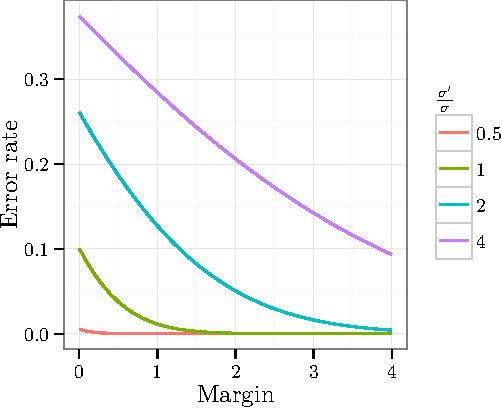
\includegraphics[width=.7\linewidth]{analysis/messina/figure/05-E1-E1A3-1}
\caption[High margin increases classifier robustness]{High margin increases a classifier's robustness to technology translation.  The class prediction error rate of a Messina2-type classifier is shown as a function of the classifier margin $\Delta$, and the noise level of a new measurement technology, $\sigma'$.  To facilitate dimensionless comparison, $\Delta$ and $\sigma'$ are shown scaled relative to the noise level $\sigma$ of the technology used to generate the Messina2 training data.}\label{fig:mess-margin-good}
\end{figure}

\subsection[Messina2 controls classifier margin]{Messina2 provides accurate control over classifier margin}
High-margin classifiers are desirable due to their robustness, but is Messina2 actually effective in building classifiers with high margin, and how does this compare to other techniques?  To address this, Messina2 and representative other techniques were applied to simulated diagnostic and prognostic data.  Methods were compared for sensitivity -- the rate at which they detected simulated biomarkers with desired characteristics -- and specificity -- the rate at which they rejected simulated biomarkers lacking desired characteristics.

\paragraph{Classification ($f_M$)}
Messina2 with an $f_M$ objective was compared to the t-test.  Simulated $x_i$ were drawn from a normal distribution, as $x_i \sim \mathcal{N}(D y_i, 1)$, with $D \in [0, 5]$ and $y \in \{0, 1\}$.  Classes were balanced, so that near-equal numbers of $y = 0$ and $y = 1$ samples were present in all runs.  The total number of samples in a run, $n$, was either 25, 50, or 100.  For each combination of $D$ and $n$, \fcardinal{1000} random cohorts were generated and supplied to Messina2 and the t-test, and detection rates recorded.  Messina2's $f_M$ parameters were $l_n \geq 0.8$, $l_c \geq 0.8$, and $\Delta \geq 1$, and the t-test size ($\alpha$) was $0.05$.

Across all sample sizes, Messina2 consistently only selected a biomarker when its true margin was near the target value of 1 (\fref{fig:mess-vs-t}).  Conversely, the t-test was far less selective, identifying even biomarkers with a zero margin as being differentially-expressed.  This sensitivity to small differences, particularly in large samples, is a concrete example of the effect illustrated in \fref{fig:messina-example-stats-class}: a statistically significant result does not necessarily indicate that a good classifier can be made.  The result of this simulation suggests that if the t-test were used to identify single-gene diagnostic biomarkers, a very high false positive rate could be expected, and many of the reported biomarkers would lead to small-margin classifiers that would be unlikely to be robust.  This effect only becomes more pronounced as the sample size increases.

\begin{figure}[!htbp]
\centering
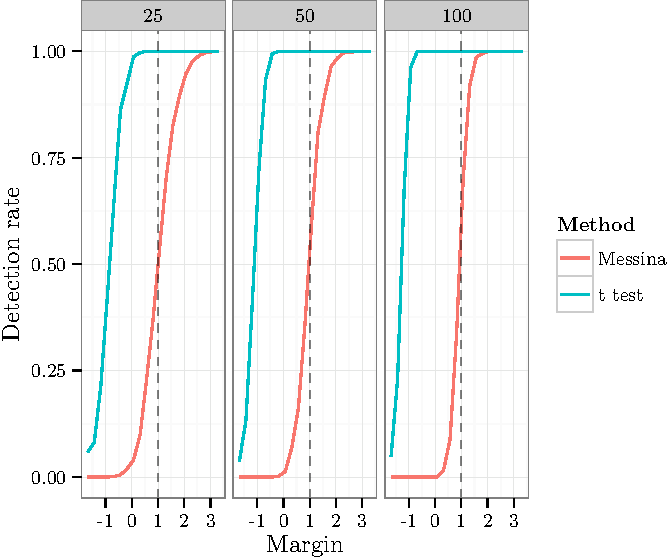
\includegraphics[width=\linewidth]{analysis/messina/figure/06-E2A-E2A-plots-1}
\caption[Messina2 $f_M$ selects only desired biomarkers]{Messina2 with $f_M$ is less sensitive, but more specific, than the t-test.  Across three sample sizes (top bars), simulated biomarker measurements for two groups were drawn from normal distributions with a range of class separations, and the rates at which Messina2 and the t-test detected a simulated biomarker were compared.  The t-test detected almost all simulated biomarkers under all conditions, even those for which the margin was zero, and robustness would likely be poor.  In contrast, Messina2 reliably only detected biomarkers with margins at least as high as its target of 1, shown as dashed vertical lines.  If the goal is to identify biomarkers that can be made into high-margin diagnostic classifiers, these results indicate that Messina2 is a far more discriminating selection method than the t-test.}\label{fig:mess-vs-t}
\end{figure}

\paragraph{Prognosis ($f_H$)}
Messina2 using the $f_H$ objective function was compared to the \texttt{maxstat} corrected optimal cut procedure, and the simple median-cut log-rank test.  Simulated data were generated in a similar fashion to the $f_M$ test above, as follows.  Simulated $x_i$ were drawn as $x_i \sim \mathcal{N}(D s_i, 1)$, with $D \in [0, 5]$, and $c_i \in \{0, 1\}$ the class membership indicator.  The fraction of class 1 in the sample was either $0.2$ or $0.5$, with number of samples $n \in \{25, 50, 100\}$.  Event times were sampled from an exponential distribution with rate $4 c_i$, and censoring times from an exponential distribution, with rate calculated to give an expected censoring rate of $0.2$~\footnote{A number of values of the censoring fraction were tested, which for reasonable levels was observed to have only minor effects on results (data not shown).}.  500 simulations were performed for each unique combination of parameters.  Messina2's $f_H$ arguments were $l_h \geq 2$ and $\Delta \geq 1$, and \texttt{maxstat} was used with test \texttt{"LogRank"} and correction method \texttt{"HL"}.  For \texttt{maxstat} and the median-cut, a biomarker was considered detected if its corrected P-value was less than $0.05$.

The detection results on these simulated data are shown in \fref{fig:mess-vs-maxstat}.  Messina2 was not as reliable at controlling classifier margin in these prognostic data as it was in the classification case (\fref{fig:mess-vs-t}); this discrepancy may be due to the greater uncertainty inherent in censored data.  Despite this, Messina2 remained competitive with the other cut optimization procedure \texttt{maxstat}, particularly in small samples.  Messina2 was also substantially faster than \texttt{maxstat}, on the test system taking $0.41$ seconds per biomarker per core for $n = 100$, versus $4.80$ seconds for \texttt{maxstat}\footnote{Messina2Core is much faster again; approximately 50 times the speed of Messina2, at default settings.}.  As expected, the median cut procedure was very sensitive when the survival subgroups were balanced, but performed poorly otherwise.

\begin{figure}[!htbp]
\centering
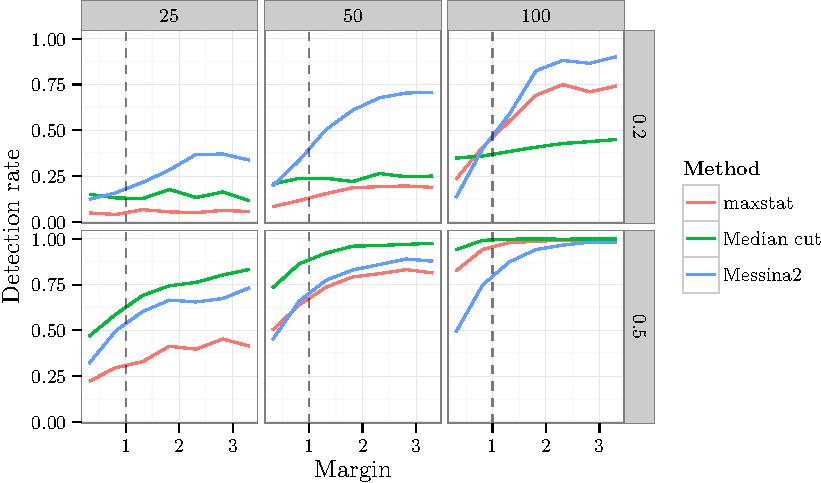
\includegraphics[width=\linewidth]{analysis/messina/figure/06-E2B-E2B-plots-1}
\caption[Messina2 prognostic performance compared to alternative methods]{Messina2 $f_H$ prognostic performance, compared to \texttt{maxstat} and median cut.  Detection rate for each method is shown as a function of margin, for sample sizes of 25, 50, and 100 samples (top bars), and class 1 proportions of $0.2$ and $0.5$ (side bars).  The target classification margin of 1 is shown as dashed vertical lines.  Although Messina2 (blue) did not control margin as effectively as in the $f_M$ classification case, it performed competitively against \texttt{maxstat} (red), particularly in the case of small sample sizes.  The median cut procedure (green) was highly sensitive when classes were balanced (class 1 proportion of $0.5$), but performed poorly otherwise.}\label{fig:mess-vs-maxstat}
\end{figure}

\subsection[Messina2 vs maxstat: prognostic classifier training]{Messina2 is more effective than maxstat at finding validating prognostic biomarkers}
The preceding simulation studies have indicated that high-margin threshold classifiers are robust to measurement noise, and that Messina2 is efficient at learning such classifiers, but the advantage of Messina2 over other methods on real data remains to be shown.  The \gls{GEX} measurements in \gls{PDAC} cohorts used in \Cref{chap:signatures} provide a platform for this comparison, by examining the rate at which a prognostic biomarker found by a given technique in one cohort, will validate as prognostic in a separate cohort.  The \gls{PDAC} cohorts contain patients from different countries, with differing clinical characteristics, and with biomarkers measured by different technologies, and so provide a strong test of the generalization ability of classifiers built by Messina2 and \texttt{maxstat}.

Pseudo-\gls{ROC} curves were generated to compare the validation performance of default Messina2, Messina2 without bootstrap (Messina2Core), and \texttt{maxstat}.  Classifiers of each type were trained on data from the \gls{APGI} \gls{PDAC} cohort, and validated on data from cohorts GSE28735, and \gls{TCGA} paad.  To generate a pseudo-\gls{ROC} curve for each method, the trained classifiers were first ranked by a quality metric (increasing margin for Messina2, decreasing P-value for \texttt{maxstat}).  Then, for each rank of the metric $r$, two values were calculated: the proportion of classifiers with rank at least as good as $r$ that did validate (the validation rate, similar to the true positive rate of a conventional \gls{ROC}), and the proportion of classifiers with rank worse than $r$ that did \emph{not} validate (the non-validation rate, similar to the false positive rate of \gls{ROC}).  The pseudo-\gls{ROC} is then the curve formed by plotting the validation rate against the non-validation rate, for all ranks of the metric.  A detailed description of the validation procedure and pseudo-ROC calculation can be found in the Methods section.

Both Messina2 and Messina2Core produced classifiers that were far more likely to validate than those returned by \texttt{maxstat} (\fref{fig:mess-val-detrel}).  Messina2Core in particular demonstrated excellent validation performance, suggesting that -- at least for the objective $f_H$ -- the increased stringency introduced by Messina2's bootstrap validation procedure came at the expense of substantial sensitivity.  For the very highest-margin classifiers, Messina2's performance was close to that of Messina2Core, indicating that the sensitivity loss is primarily restricted to lower-margin biomarkers.  \texttt{maxstat} gave very disappointing performance in general, with validation performance only marginally better than that of random selection, emphasising the robustness of classifiers generated from a machine learning perspective, rather than a statistical one.

\begin{figure}[!htbp]
\centering
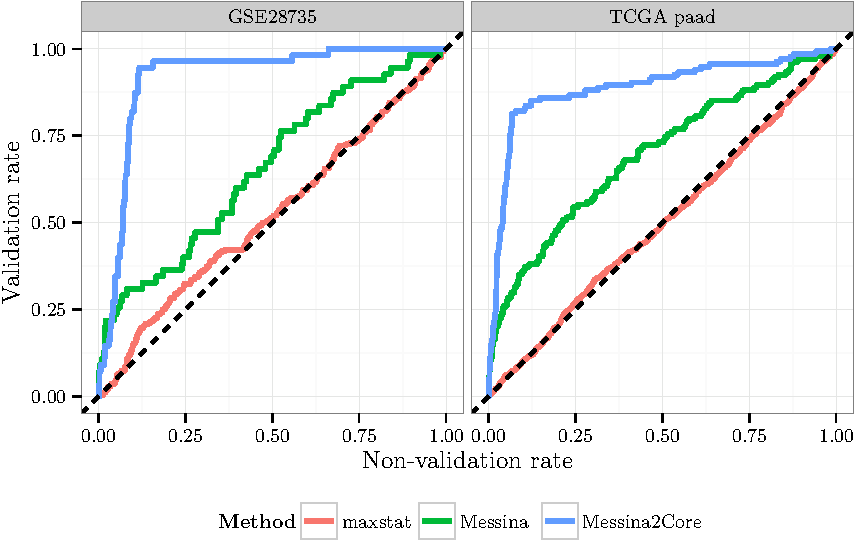
\includegraphics[width=\linewidth]{analysis/messina/figure/07-E3-E3-val-detcurves-plots-1}
\caption[Validation performance of Messina2 versus \texorpdfstring{\texttt{maxstat}}{maxstat}]{Messina2 identifies classifiers much more likely to validate than those found by \texttt{maxstat}.  Pseudo-ROC curves (see accompanying discussion and methods for a more complete description of these curves) are shown comparing the validation performance of classifiers found by applying Messina2, Messina2Core, and \texttt{maxstat}.  Classifiers were trained on the \gls{APGI} \gls{PDAC} cohort, and then tested in validation cohorts GSE28735, and \gls{TCGA} paad.  Messina2Core demonstrates excellent performance, being able to effectively separate validating classifiers from non-validating classifiers in both cohorts.  Messina2 was as sensitive as Messina2Core for high-margin classifers (bottom left of the graphs), but showed greatly diminished sensitivity for lower margin classifiers.  \texttt{maxstat} was barely better than random, and overall performed very poorly for the generation of classifiers that would be likely to validate in external cohorts measured by different technologies.  The dotted line with slope $0.5$ indicates the performance expected from random selection of biomarkers.}
\label{fig:mess-val-detrel}
\end{figure}


\subsection[Messina2 identifies candidate \texorpdfstring{\acrshort{PDAC}}{PDAC} biomarkers]{Application of Messina2 to identify biomarkers for \texorpdfstring{\acrshort{PDAC}}{PDAC} prognosis}
The very promising results of Messina2 in pseudo-ROC analysis prompted its use in the \gls{APGI} \gls{PDAC} cohort, to identify new prognostic biomarkers for use in a preoperative prognostic tool like that developed in \Cref{chap:nomogram}.  Messina2 was used to identify prognostic biomarkers in the \gls{APGI} \gls{GEX} and follow-up data described in \Cref{chap:signatures}, using objective function $f_H$ with $l_h = 2$, and $\Delta \geq 1$.  Of \fcardinal{13000} mRNAs tested, three passed these requirements (\tref{tab:mess-apgi-leads}).  The genes associated with these mRNAs have been reported to be linked to cancer: KRT6A and KRT6C are associated with poor prognosis basal cancers~\cite{Choi2014,Livasy2006}, KRT6A in particular has been linked to poor prognosis in \gls{PDAC}~\cite{VandenBroeck2012}, and ANGPTL4 is involved in metastasis in a range of cancers~\cite{Adhikary2013,Kim2011b,Padua2008,Xiao2012}.

\begin{table}[!htb]
\centering
\caption[Outcome-associated biomarkers found by Messina2 in the \texorpdfstring{\acrshort{APGI}}{APGI} \texorpdfstring{\acrshort{PDAC}}{PDAC} cohort]{High-margin outcome-associated biomarkers found by Messina2 in the \acrshort{APGI} \acrshort{PDAC} cohort.}
\label{tab:mess-apgi-leads}
\begin{tabular}{@{}llll@{}}
\toprule
Gene    & Threshold ($t^*$) & Direction ($d^*$) & Margin ($\Delta^*$) \\ \midrule
KRT6A   & 9.50              & 1                 & 2.00                \\
ANGPTL4 & 8.90              & 1                 & 1.36                \\
KRT6C   & 7.46              & 1                 & 1.17                \\
\bottomrule
\end{tabular}
\end{table}

TODO figures

The Messina2 classifiers of \tref{tab:mess-apgi-leads}, trained on the \gls{APGI} cohort, were tested for prognostic differentiation in the GSE28735 and \gls{TCGA} paad validation cohorts, but none produced sample groupings with significantly different prognosis (Four log-rank tests, as not all genes of \tref{tab:mess-apgi-leads} were present in the validation cohorts, all $\chi^2 < 1.64$).  This lack of validation, while disappointing, is quite plausibly due to small cohort size (TCGA), microarray probe dropout (GSE28735), or simply the very small number of genes tested, and more involved validation (by immunohistochemistry, for example) may prove fruitful.

\section{Discussion}
The thesis driving this work was that ``large margin binary decision stump classifiers can provide a principled way to translate research biomarker measurement data into simple but high-performance clinical tests.''  Confirming this hypothesis, the preceding sections have established the robustness of Messina2's classifiers for both diagnosis and prognosis, showed that Messina2 provides control over classifier margin, and demonstrated on real data that Messina2 represents a principled way to select classifiers with a high likelihood of validating in external cohorts.  These capabilities of Messina2 are -- as far as I am aware -- unique, and Messina2 shows promise for the much-needed identification of more effective prognostic biomarkers in \gls{PDAC}.  One of the particular strengths of Messina2 is its great generality, and through user-supplied objective functions Messina can be used to learn effectively any type of binary separation.  Messina2's most salient limitation at this time is its restriction to univariate binary classifiers; relaxing these restrictions may improve performance and detection rate, although computational issues may make this infeasible.

Direct simulation and the \gls{PDAC} validation demonstrated that high-margin Messina2 classifiers were more robust to the inflation in measurement noise that may come with technology translation.  In additional work not shown here, classifiers with large margins were also found to be more resistant to the differences in measurement slope and intercept that accompany poor calibration.  The low error rate and high robustness of large-margin classifiers is intuitively reasonable, and has strong theoretical support~\cite{Vapnik2000}, making methods capable of controlling classifier margin important tools in designing robust biomarker-based clinical tests.

In simulation experiments, Messina2 $f_M$ provided highly accurate control of the classifier margin, allowing the analyst to confidently train large-margin diagnostic classifiers with a high likelihood of validating in external data.  This capability is unique to Messina2: competing univariate test-based methods of biomarker selection do not control for margin size, and in a classification context are likely to have an unacceptably high non-validation rate (\fref{fig:mess-vs-t}).  In contrast to the $f_M$ case, Messina2 $f_H$ provided poor control over classifier margin, although it was generally competitive with alternate approaches (\fref{fig:mess-vs-maxstat}).  The relatively poor selectivity of Messina2 $f_H$ may simply be a consequence of the greater uncertainty encountered in outcome data, but warrants further investigation.  In both the diagnosis and prognosis contexts, it can be argued that univariate statistical tests can still be used to achieve a form of margin control, through increasing the stringency of P-value selection.  Although this will indirectly lead to margin improvements, a remaining issues with univariate test selection methods is that they can not integrate asymmetric costs, or more complex selection criteria, while still optimizing margin.  Asymmetric cost is very commonly encountered in medical decision making~\cite{Pepe2001}, and the utility of univariate test methods in clinical test development is severely limited by their inability to perform cost-sensitive selection.

Messina2's use of general objective functions gives it immense flexibility.  Two example objectives have been presented, $f_M$ for cost-sensitive classification, and $f_H$ for prognosis, but any objective that can be adapted into the binary separation framework can be optimized by Messina2.  This generality represents a distinct advantage of Messina2 over machine-learning techniques, which usually\footnote{The only exception of which the author is aware is nearest neighbour techniques, which can be completely agnostic of the domain $\mathbb{Y}$.} require bespoke adaptation to a new predicted variable domain.

When applied to real data reflecting a translation scenario, Messina2 demonstrated excellent performance in identifying biomarkers that would validate in external cohorts (\fref{fig:mess-val-detrel}).  The sensitivity of both Messina2, and Messina2Core, was far superior to that of the competing biomarker selection technique \texttt{maxstat}, with Messina2Core performing particularly well.  Messina2Core lacks the bootstrap validation step used by Messina2, and the large difference in sensitivity between the two techniques indicates that Messina2's higher stringency comes at the expense of great sensitivity.  However, it is notable that for the most specific bottom-left region of the pseudo-\gls{ROC} curves of \fref{fig:mess-val-detrel}, Messina2 and Messina2Core show similar performance.  This region is the one that is of most interest during classifier development, and so the lower sensitivity of Messina2 away from this region is of little practical consequence.  The very poor performance of \texttt{maxstat} was surprising, with the technique constructing classifiers that validated little better than chance, and was particularly puzzling given the competitive performance of \texttt{maxstat} in simulation studies (\fref{fig:mess-vs-maxstat}).  The huge divide in validation performance between the Messina2 classifiers, and the \texttt{maxstat} method, may well reflect again the divide between statistical significance and classifier performance (\fref{fig:messina-example-stats-class}): although \texttt{maxstat} is an effective statistical test for differential survival, it is a poor method for the construction of actual prognostic classifiers.

The work of \Cref{chap:nomogram} investigated the use prognostic biomarkers to predict survival with resected \gls{PDAC}, with underwhelming results.  It could be that \gls{PDAC} is a disease with a fundamentally unpredictable course -- although the results of \Cref{chap:signatures} suggest that this is not the case -- or the biomarkers used in \Cref{chap:nomogram} may simply be poor markers of outcome.  To identify potential better biomarkers of \gls{PDAC} prognosis following resection, Messina2 was applied to data from the \gls{APGI} \gls{PDAC} cohort.  Three high-margin genes were identified TODO fig link -- KRT6A, ANGPTL4, and KRT6C -- all with plausible literature connections to outcome with \gls{PDAC}~\cite{Adhikary2013,Choi2014,Kim2011b,Livasy2006,Padua2008,VandenBroeck2012,Xiao2012}.  Unfortunately, none of the three biomarkers validated on either of the GSE28735, or the \gls{TCGA} paad cohorts.  This disappointing result may be due to technical effects, and a more careful validation of these three markers is certainly warranted, given their strong literature ties to outcome and metastasis.  Although, given more complete data, better single-gene biomarkers of prognosis will likely be found in \gls{PDAC}, the orthogonal metagene result of \Cref{chap:signatures} suggests that optimal prognosis will require a variant of Messina that can work with joint biomarker distributions.

Messina2's greatest limitation is its restriction to examining biomarkers singly.  This was a practical choice made for a number of reasons: it vastly restricts the classifier search space, reduces the quantity of data required for stable fitting, and matches well the clinical desire for classifiers that use as few biomarkers as possible.  However, these benefits come at the cost of prediction performance: with a Vapnik-Chervonenkis dimension~\cite{Vapnik2000} of 2, Messina2 classifiers are capable of learning only extremely simple data patterns.  There is evidence that excellent classification performance can be achieved from measurement of only a few biomarkers~\cite{Grate2005}; this is still a small enough number to be attractive as a clinical diagnostic, and could potentially provide large gains in performance over Messina2.  However, the issues of computational tractability, and stability in reasonable-sized data sets, remain.  Very little work has been done in this direction, and it remains an area for future development.


\section{Methods}

\subsection{Messina2 version}
The version of Messina2 used in this chapter is implemented in the \texttt{R} environment, and is available as the \texttt{thesis} branch in the Bitbucket repository \texttt{marpin/r-messina}.  This can be directly installed from an instance of \texttt{R} that has the \texttt{devtools} package installed, by running the command \texttt{devtools::install\_bitbucket("marpin/r-messina", ref = "thesis")}.

\subsection{Simulation studies}
Simulation experiments were as described in the text.  All calculations were performed in the \texttt{R} environment.

\subsection{\texorpdfstring{\acrshort{PDAC}}{PDAC} data}
\gls{PDAC} \gls{GEX} and outcome data were from the \gls{APGI}, \gls{TCGA} paad, and GSE28735 cohorts, following unsupervised selection, processed as described in \Cref{chap:signatures}.

\subsection{Pseudo-\texorpdfstring{\acrshort{ROC}}{ROC} generation}
A pseudo-\gls{ROC} curve for a given training technique and validation cohort was calculated as follows.

The training technique was applied to the \gls{APGI} \gls{PDAC} \gls{GEX}-outcome data, to yield a list of threshold prognostic classifiers.  This list was then sorted in order of decreasing classifier figure of merit.  For Messina2 and MessinaSurv, this figure of merit was the margin, $\Delta^*$; for \texttt{maxstat}, this was the negative of the classifier P-value.  Classifiers based on transcripts which were not present in the validation data were discarded from the list.  Each classifier in the list was then tested for prognostic significance in the validation set.  This was achieved by first affinely scaling the optimal classifier threshold $t^*$, which based on the distribution of biomarker measurements in the \gls{APGI} training data, to approximately match the distribution of measurements in the validation data, as follows: 
\begin{equation*}
t'^* = \left(t^* - \mu(x)\right)\frac{\sigma(x')}{\sigma(x)} + \mu(x')
\end{equation*}
where $t'^*$ is the threshold to be used on validation data; $x$ is the \gls{APGI} training data, and $x'$ the validation data, for the biomarker under consideration; and $\mu$ and $\sigma$ are the $\tau$-estimators of location and scale~\cite{Maronna2002}, as implemented in the \texttt{R} package \texttt{robustbase}.  The scaled $t'^*$  was then used to partition the validation data into two subgroups, defined by $w'_i = [x'_i \geq t'^*]$, and a log-rank test for differences in outcome between the groups $w = 0$ and $w = 1$ was performed.  The classifier was considered to have validated if the uncorrected test P-value was less than $0.05$.

To plot the pseudo-\gls{ROC} curve, for each classifier in the sorted list, two quantities were calculated.  The first was the true validation rate, which was the fraction of classifiers with figure of merit at least as good as the classifier under consideration, that did validate; the second was the false validation rate, being the fraction of classifiers with figure of merit at least as good as the  classifier under consideration, that did not validate.  A plot of the true validation rate versus the false validation rate, for all figures of merit, yielded the pseudo-\gls{ROC} curve.

Pseudo-\gls{ROC} curves were calculated for three training techniques: Messina2 ($f_H$ with $l_h \geq 2$ and $\Delta^* \geq 1$), Messina2Core (parameters as for Messina2), and \texttt{maxstat} (test \texttt{"LogRank"}, correction method \texttt{"HL"}); and two validation cohorts: \gls{TCGA} paad, and GSE28735.

\section{Attribution}
The conception and planning of this project, and all work, was performed solely by me.

\end{document}
